\section{Paket-Anzahldurchschnitt der 10 beliebtesten JavaScript-Github-Repositories} \label{sec:PackageMeanPopGitJsRepos}
    \begin{figure}[H]
        \centering
        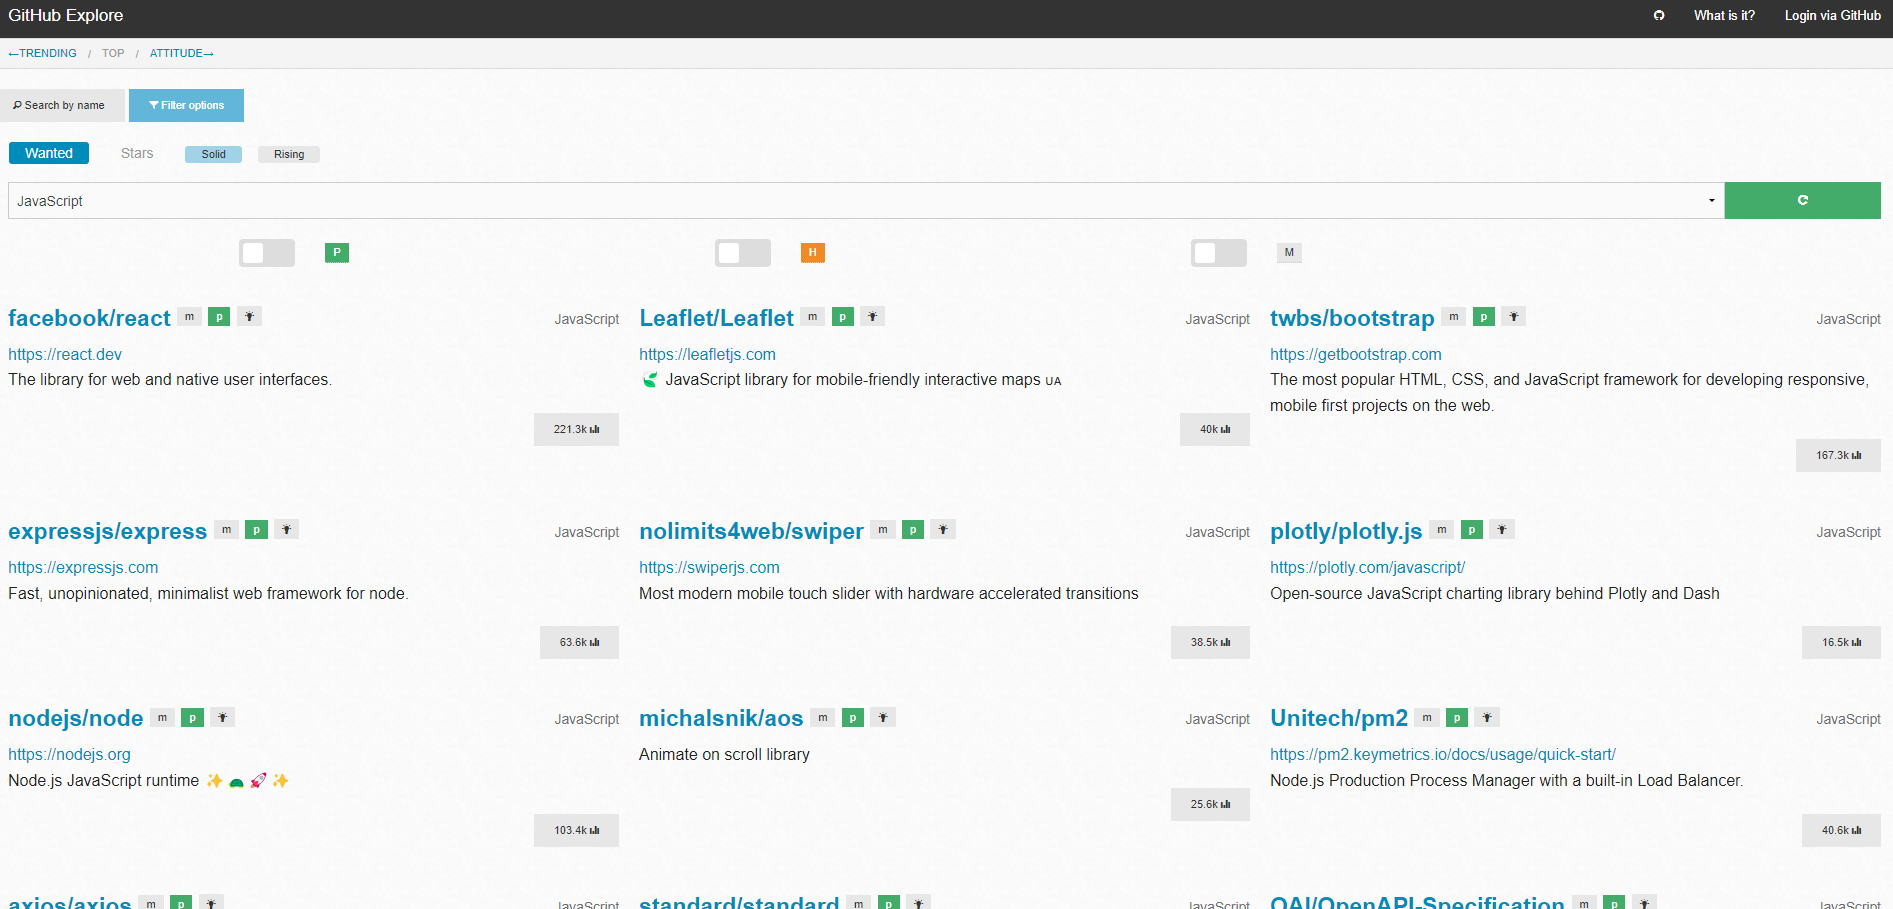
\includegraphics[width=0.85\textwidth]{Appendix/gitmost_wanted_2024-04-29 181855.png}
        \caption{Quellen: \cite{link:GitPopJsRepoMostWanted}}
        \label{png:gitMostWanted}
    \end{figure}
    Dort dann folgende Repositories: \cite{link:GitPopJsRepoReact}, \cite{link:GitPopJsRepoLeaflet}, \cite{link:GitPopJsRepoBootstrap}, \cite{link:GitPopJsRepoExpress}, \cite{link:GitPopJsRepoSwiper}, \cite{link:GitPopJsRepoPlotly}, \cite{link:GitPopJsRepoNode}, \cite{link:GitPopJsRepoAos}, \cite{link:GitPopJsRepoPm2}, \cite{link:GitPopJsRepoAxios}
    \begin{eqnarray}
        16.085 + 678 + 974 + 54 + 788 + 1.815 + 488 + 688 + 241 + 1.768 &=& 24.299
        \label{eq:summe} \\
        \frac{24.299}{10} &=& 2.429,9
        \label{eq:mean}
    \end{eqnarray}
    Somit beträgt das arithmetische Mittel der Abhängigkeiten der 10 beliebtesten Git-Repositories laut \eqref{eq:mean} $2.429,9$ Pakete.
